\documentclass[12pt]{article}
\usepackage[utf8]{inputenc}
\usepackage{graphicx}
\usepackage{float}
\usepackage{amsmath}
\usepackage{placeins}
\usepackage{gensymb}


\usepackage[letterpaper,margin=0.75in]{geometry}
\graphicspath{images/}
\begin{document}
\begin{titlepage}
\begin{center}
% Upper part of the page
\vbox{}
\vbox{}
\vbox{}
\vbox{}
\vbox{}
\vbox{}
\vbox{}
\vbox{}
\vbox{}

\includegraphics[width=0.75\textwidth]{Images/ubc.png}\\[0.5cm]
\textrm{Martin Alejo}\\[0.5cm]
\catcode`#=12
\textrm{#75296665}\\[0.5cm]
\textrm{December 9, 2022}\\[0.5cm]
\textrm{Mini Project 4}\\[0.5cm]
\textrm{University of British Columbia}\\[0.5cm]
\textrm{Electrical and Computer Engineering}\\[0.5cm]
\textrm{ELEC 301}\\[0.5cm]
\textrm{Instructor: Nicolas Jaeger}\\[0.5cm]

\includegraphics[width=0.18\textwidth]{Images/Signature.png}\\[0.5cm]
\vbox{ }
\end{center}
\end{titlepage}
\pagebreak
\pagenumbering{roman}
\tableofcontents
\pagebreak
\listoffigures
\listoftables
\pagebreak
\pagenumbering{arabic}


\section{Introduction}
For this project, we will be using SPICE software to simulate active filters and oscillators.
\section{Part A}
For this part, we will be designing a 2nd order Butterworth low pass active filter using the UA741 operational amplifier. 

Here is the circuit that we will be using for this part:

\begin{figure}[H]
    \centering
    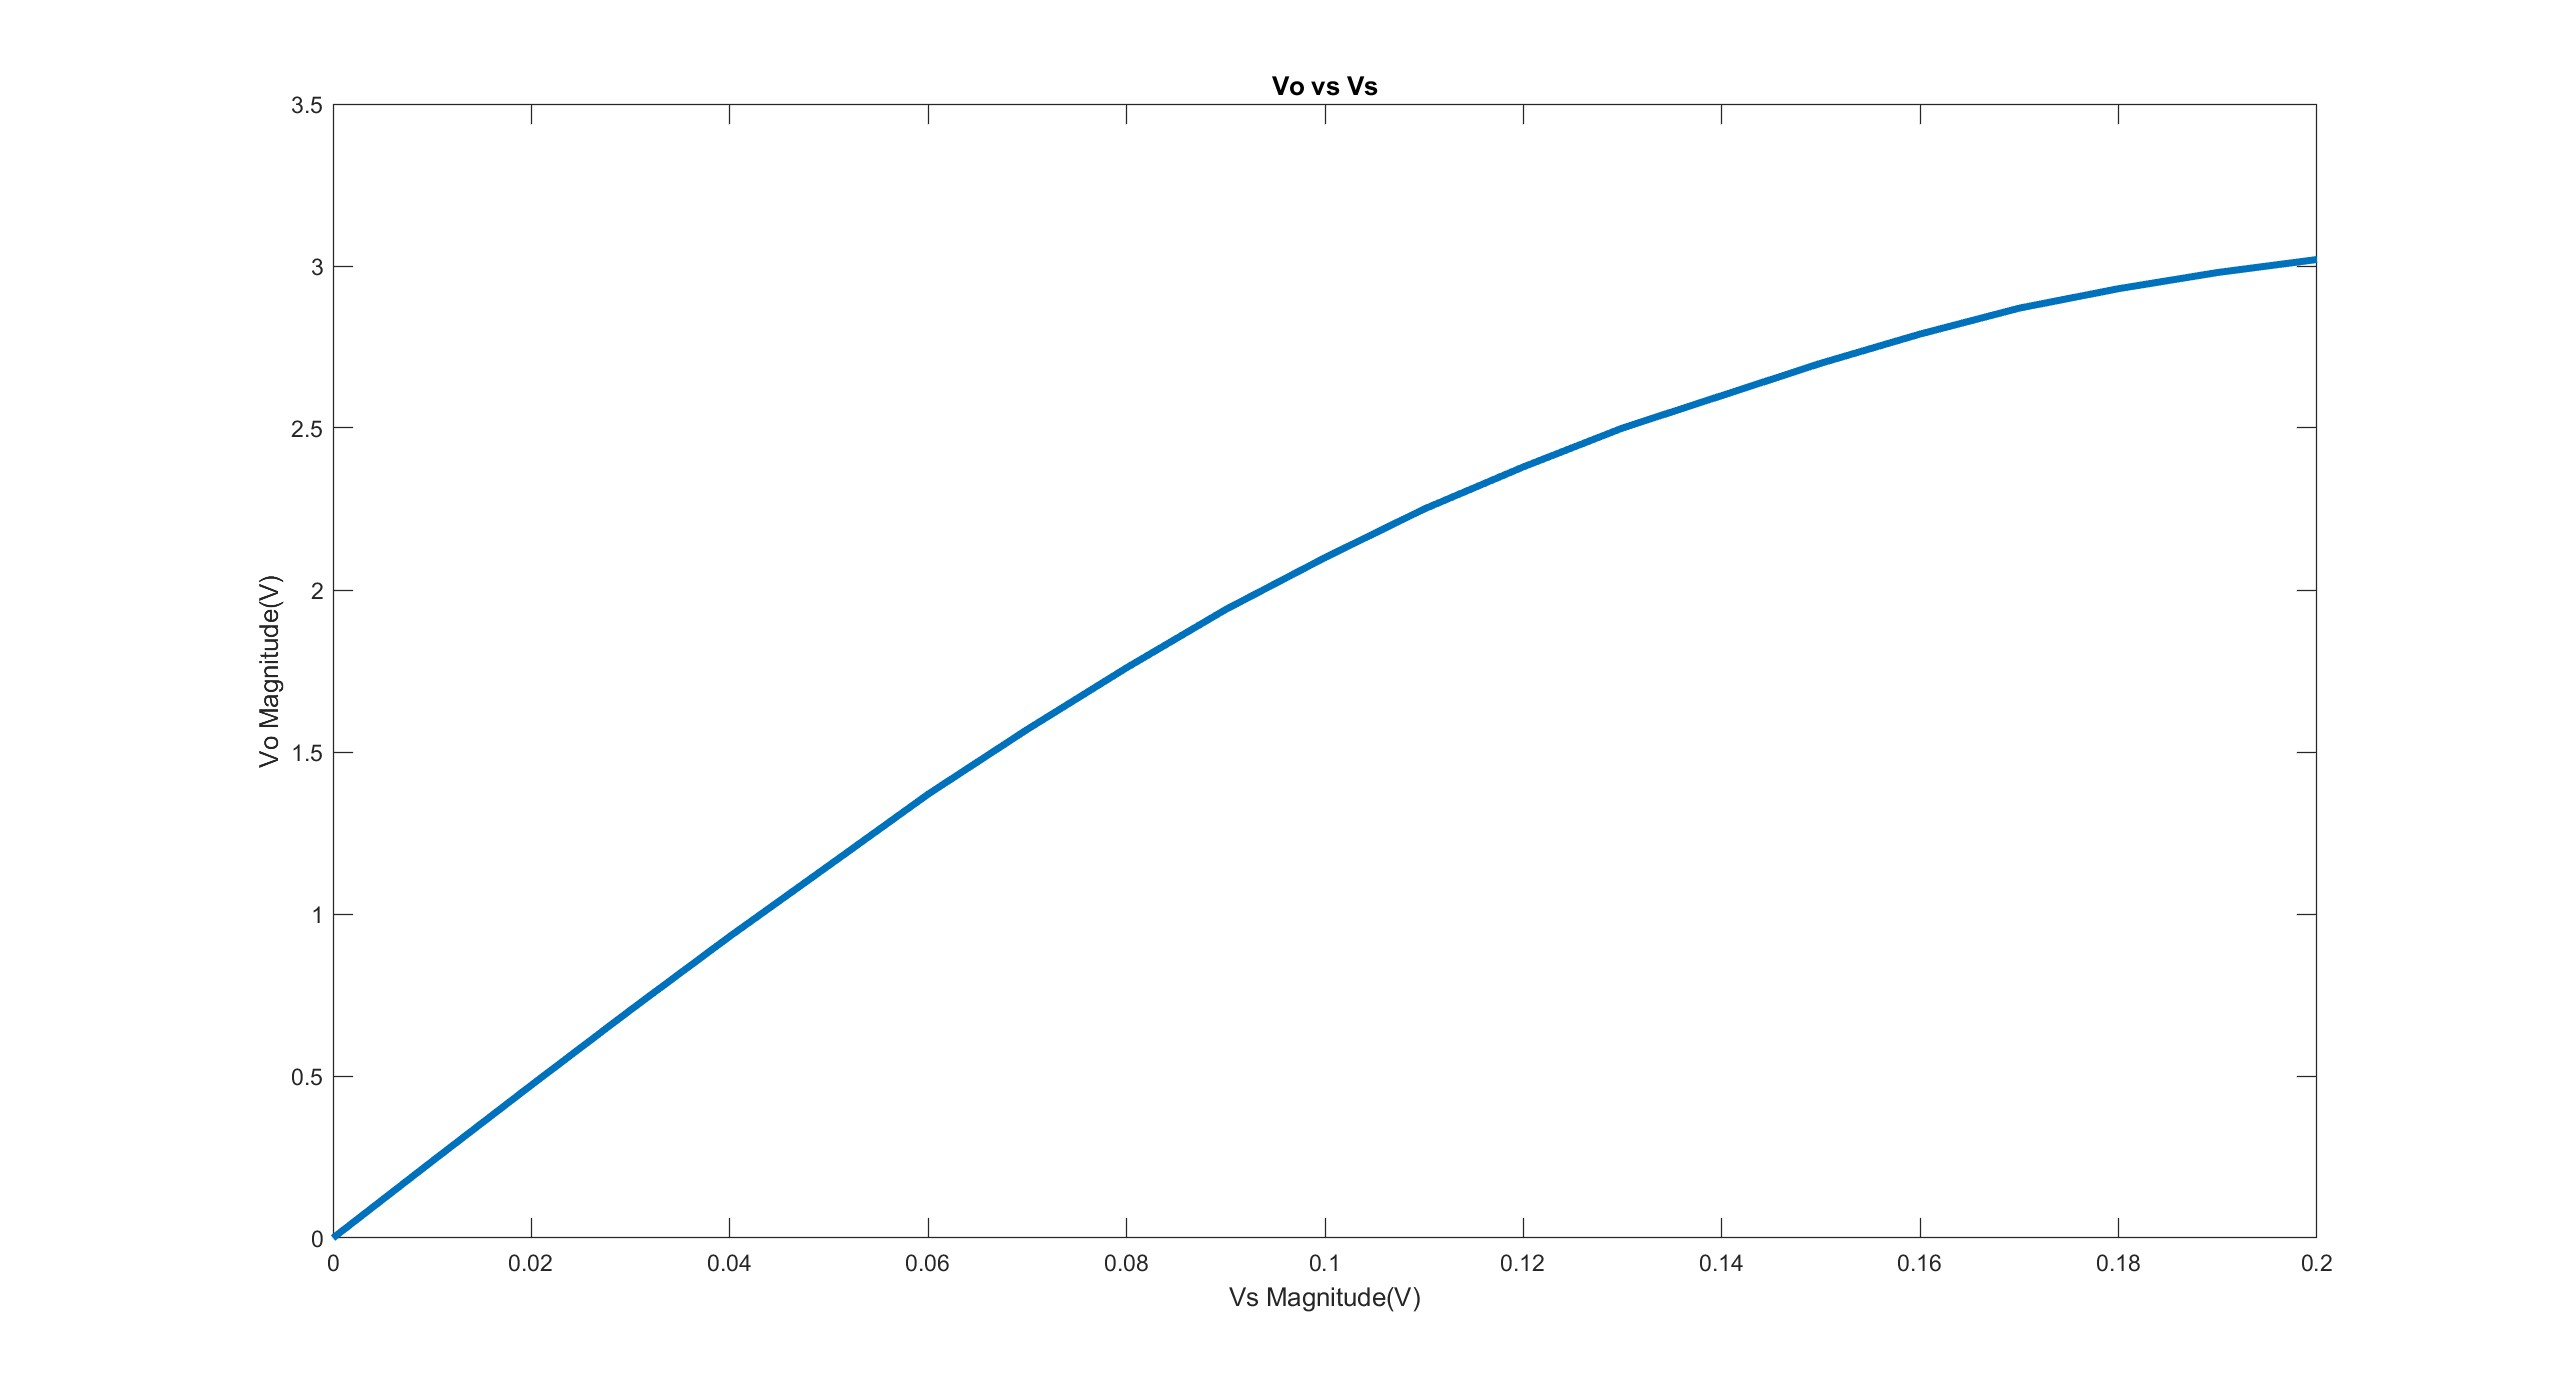
\includegraphics[height=0.5\textwidth]{Images/voltage_transfer_plot_2N2222A.jpg}\\
    \caption{Second Order Butterworth Filter}
    \label{fig:transfer_plot_2N2222A}
\end{figure}
The calculations to find the resistance $R_1$,$R_2$ and capacitance C, we will be using the formulas from the class notes [1].  
\section{Part B}


\section{Part C}

\section{References}
1. ELEC 301 Class notes 
\newline
2. Mini Project 4 Document
\newline
3. Standard Resistor and Capacitor Values (Canvas)
\newline
4. Circuit Maker SPICE Model


\end{document}